\documentclass[a4]{scrartcl}

\usepackage[ngerman]{babel}
\usepackage[utf8]{inputenc}
\usepackage{mathtools}
\usepackage{amsmath}
\usepackage{amssymb}
\usepackage{geometry}
\usepackage{scrpage2}
\pagestyle{scrheadings}
\clearscrheadfoot


\geometry{
  paper=a4paper, % Change to letterpaper for US letter
  top=2cm, % Top margin
  bottom=1.5cm, % Bottom margin
  left=2cm, % Left margin
  right=3cm, % Right margin
  %showframe, % Uncomment to show how the type block is set on the page
}

\setlength{\parindent}{0em}

\ohead{\\
Pina Kolling}

\begin{document}

\subsection*{Vorlesung 4}

\textbf{Potenziale von IT - Traditionelle Perspektive}

\begin{itemize}
\item unstrukturierte Abläufe in routinemäßige Arbeit überführen
\item Beschleunigung
\item Ersatz und Reduktion menschlicher Arbeit
\item Transport von Informationen mit großer Geschwindigkeit über große Entfernungen
\item große Menge von Informationen verfügbar machen
\end{itemize}

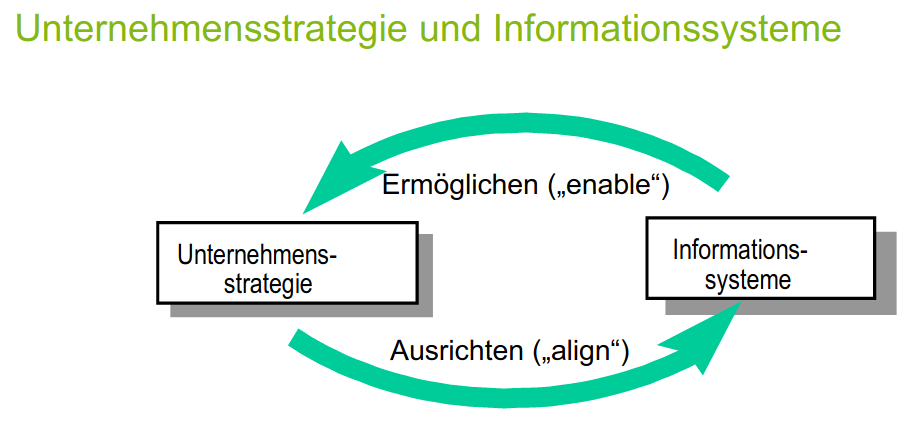
\includegraphics[scale=0.3]{UIS.png}
\\
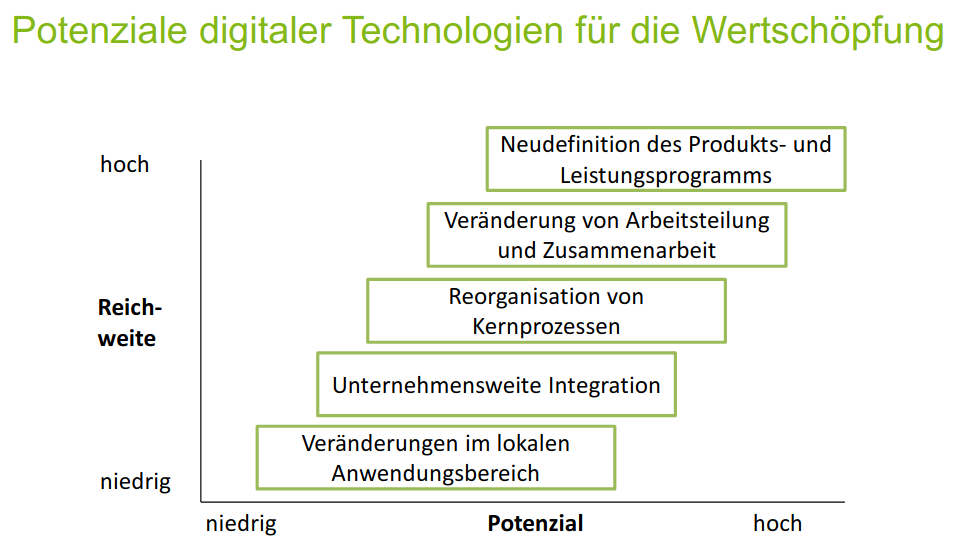
\includegraphics[scale=0.3]{Potenziale.png}

\ \\

\textbf{Digitale Transformation - Zentrale Schritte}

\begin{itemize}
\item Starke operationale Grundlage: \\
Zuverlässige Kunden- und Produktdaten, End-to-End Transaktionsprozesse, Transparenz bei Kundentransaktionen

\item Experimentierfreudigkeit: \\
Umfassende Einbindung von Mitarbeiter in Innovationsbemühungen

\item Datengesteuerte Entscheidungskultur: \\
Hypothesenbildung, Datensammlung und detaillierte Auswertung, Top-Level Entscheidungskultur

\item Digitale Angebotsplattform: \\
Wiederverwendbare Datentools und Algorithmen, Unterstützung bei der Konfiguration digitaler Lösungen

\end{itemize}

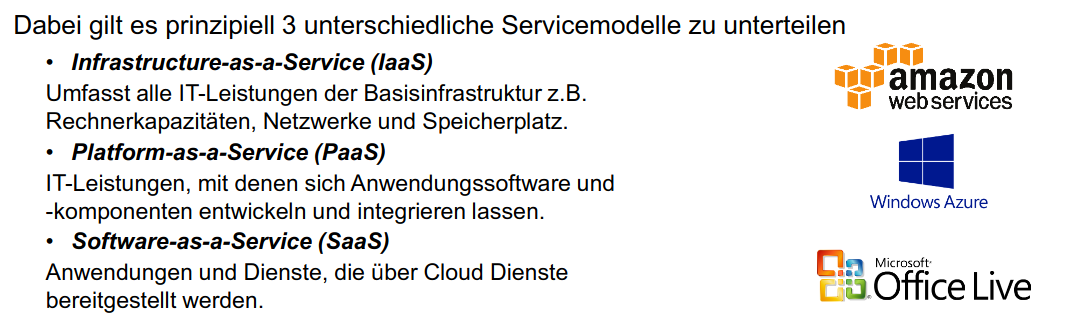
\includegraphics[scale=0.4]{repeat.png}

\ \\

\textbf{Internet of Things}
\begin{itemize}
\item neben klassischen Rechnern und mobilen Endgeräten werden auch beliebige physische Gegenstände eingebunden
\end{itemize}

\ \\
\textbf{Augmented Reality}
\begin{itemize}
\item erweiterte Realität
\item computergestützte Erweiterung der Realitätswahrnehmung
\item Beispiel: mit App und Kamera Möbel virtuell in physischem Zimmer platzieren
\end{itemize}
\ \\

\textbf{Blockchain}
\begin{itemize}
\item Liste von Datensätzen (verteilte, öffentliche Datenbank)
\item dezentral verwaltet $\rightarrow$ sicher
\item Blöcke werden miteinander verkettet
\end{itemize}

\ \\

\textbf{Kerneigenschaften digitaler Technologien}
\begin{itemize}
\item Homogenität der Daten
\item Re-Programmierbarkeit
\item Selbstreferenzierung
\end{itemize}
 \ \\

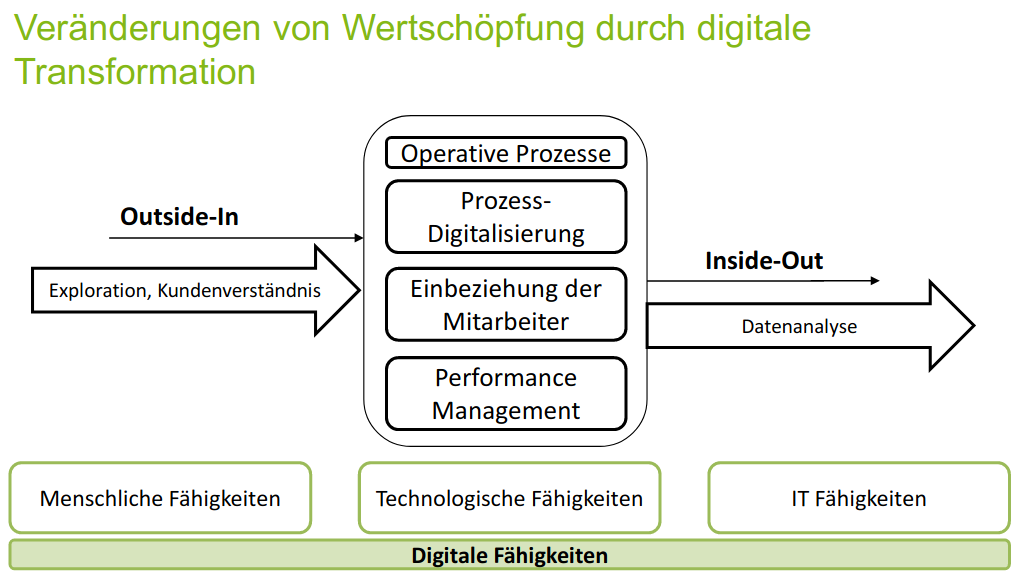
\includegraphics[scale=0.3]{veraenderung.png}


\newpage

\textbf{Digitale Fertigkeiten eines Unternehmens}
\begin{itemize}
\item Homogenität der Daten
\item Re-Programmierbarkeit
\item Selbstreferenzierung
\end{itemize}
 \ \\
 
 
\textbf{Digitale Fähigkeiten eines Unternehmens}
\begin{itemize}
\item IT-Unternehmenspartnerschaften
\item Externe IT-Verbindungen
\item Strategische Ausrichtung der IT
\item IT Geschäftsprozessintegration
\item IT Management
\item IT Infrastruktur
\end{itemize}
 
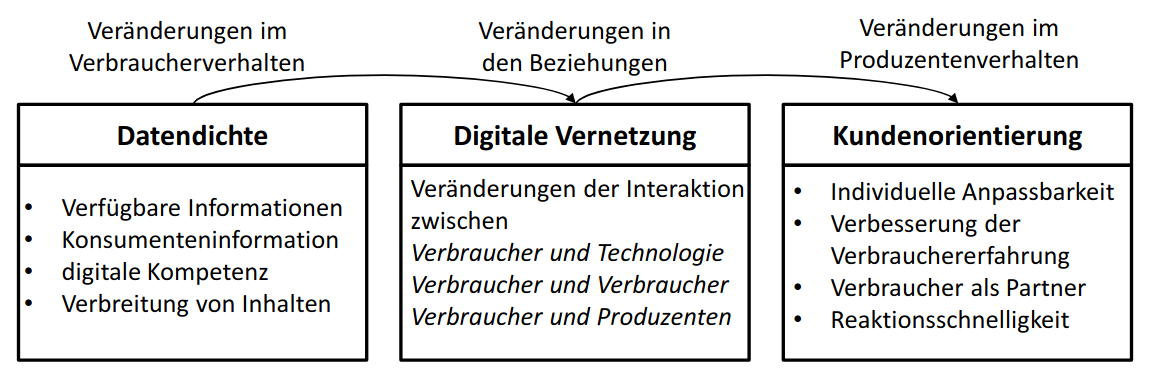
\includegraphics[scale=0.3]{prozess.png}



\textbf{Modulare Architekturen}

\begin{itemize}
\item Aufteilung eines Produktes in Module $\rightarrow$ möglichst unabhängig
\item Flexibilität, da Module unabhängig voneinander verändert oder erneuert werden können
\end{itemize}

\ \\

\textbf{Consumerization}
\begin{itemize}
\item Definition aus Vorlesung: \\
Consumerization bezeichnet den spezifischen Einfluss, den verbraucherorientierte Technologien auf Unternehmen haben können. Sie spiegelt wider, wie Unternehmen von neuen Technologien und Modellen, die aus dem Konsumbereich und nicht aus dem Unternehmens-IT-Sektor stammen, beeinflusst werden und diese nutzen können.
\item Wikipedia: \\
Consumerization bezeichnet den Prozess bzw. die Erscheinung, dass elektronische Endgeräte, wie beispielsweise Smartphone, Tablet-PCs, von Arbeitnehmern auch für ihre Erwerbsarbeit benutzt werden.
\end{itemize}

\begin{minipage}[t]{0.5\textwidth}

\textbf{Vorteile Consumerization} 
\begin{itemize}
\item bestimmte Arbeiten lassen sich dezentralisieren und flexibler organisieren und durchführen
\item mehr Kontrolle der Arbeitnehmer über ihre Zeit und Arbeitsbeziehungen
\end{itemize}

\end{minipage}\begin{minipage}[t]{0.5\textwidth}

\textbf{Nachteile Consumerization} 
\begin{itemize}
\item auflösende Grenze zwischen Berufs- und Privatleben
\item geringere Kontrollmöglichkeiten der Unternehmen
\item Firmen können über die Netzwerkverbindungen auf die privat genutzten Geräte zugreifen
\item Sicherheitsprobleme
\end{itemize}


\end{minipage}







\end{document}






